\documentclass[conference]{IEEEtran}
\IEEEoverridecommandlockouts

\usepackage{cite}
\usepackage{amsmath,amssymb,amsfonts}
\usepackage{algorithmic}
\usepackage{graphicx}
\usepackage{textcomp}
\usepackage{xcolor}
\usepackage{booktabs}
\usepackage{array}
\usepackage{hyperref}
\hypersetup{colorlinks=true,linkcolor=blue,citecolor=blue,urlcolor=blue}

\def\BibTeX{{\rm B\kern-.05em{\sc i\kern-.025em b}\kern-.08em
    T\kern-.1667em\lower.7ex\hbox{E}\kern-.125emX}}

\begin{document}

\title{Beyond the Hazard Ratio: A Causal-Inference Re-analysis of the Moertel 1990 Adjuvant Colon Cancer Trial%
\thanks{Course project for Causal Inference (Adam Kelleher, Columbia University, Spring 2026). Code and replication package: \url{https://github.com/rishika1099/Moertel-Colon-Cancer-Causal-Inference}.}}

\author{\IEEEauthorblockN{Rishika Mamidibathula}
\IEEEauthorblockA{\textit{Department of Statistics} \\
\textit{Columbia University}\\
New York, NY, USA \\
rm4318@columbia.edu}}

\maketitle

\begin{abstract}
We re-analyze the Moertel et al.\ NEJM 1990 trial of levamisole plus 5-fluorouracil (Lev+5FU) in resected stage B/C colon cancer ($n{=}929$) through five nested causal questions: the randomized average treatment effect (ATE); a back-door-adjusted ATE that pretends randomization is unknown, including a deliberate ``bad-control'' anti-example that conditions on the recurrence mediator; the conditional ATE surface across baseline covariates; the natural direct/indirect decomposition through recurrence; and transportability to a synthetic SEER 1990 stage B/C target. Every estimand is committed in $do(\cdot)$ or potential-outcomes notation \emph{before} any estimator is run, with both graphical and non-graphical identification arguments stated separately. We reproduce Moertel's headline hazard ratio of $0.67$ (we obtain $0.69$, 95\% CI $0.55$--$0.87$). The bad-control anti-example flips the apparent HR from $0.69$ to $1.10$, an unambiguous illustration of post-treatment collider bias. The natural indirect effect through recurrence prevention ($\mathrm{NIE} = +0.29$ 5-year RMST years) is extremely robust to Imai-$\rho$ sensitivity across $[-0.95, 0.95]$, while the natural direct effect is small with CI covering zero: Lev+5FU operates essentially through recurrence prevention. Transport to a synthetic SEER 1990 target shifts the HR modestly toward the null ($0.69 \to 0.71$) with a Dahabreh tipping $\mathrm{HR}_U$ of $2.75$. We argue this kind of estimand-first re-analysis should be the norm for high-stakes trials.
\end{abstract}

\begin{IEEEkeywords}
causal inference, survival analysis, mediation, transportability, sensitivity analysis, colon cancer, randomized clinical trial
\end{IEEEkeywords}

\section{Introduction}

The Moertel et al.\ trial \cite{moertel1990} established adjuvant levamisole + 5-fluorouracil (Lev+5FU) as the first effective post-operative chemotherapy for resected stage B/C colon cancer. The headline statistic --- a 33\% reduction in death hazard, $\mathrm{HR} \approx 0.67$ --- appears in every modern oncology textbook. The number is correct but causally incomplete: it elides the identifying assumptions, the absolute-scale benefit, the heterogeneity across patients, the mechanism, and the population to which the result applies.

This work re-analyzes the same data through five nested causal questions, summarized in Table~\ref{tab:questions}. Each question's estimand, 2$\times$2 cell (statistical/causal $\times$ selection/no-selection), identification assumption (graphical and non-graphical, stated separately), estimator, failure mode, and target population are committed to writing \emph{before} the corresponding estimator is run, following the contract style of Kelleher \cite{kelleher2026}. The contract document and the resulting analysis notebooks are versioned together in a public repository.

\begin{table}[t]
\caption{The five nested causal questions}
\label{tab:questions}
\centering
\renewcommand{\arraystretch}{1.15}
\begin{tabular}{@{}clp{3.0cm}@{}}
\toprule
\textbf{Q} & \textbf{Question} & \textbf{2$\times$2 cell} \\
\midrule
Q1 & Randomized ATE                & Causal $\times$ no-selection \\
Q2 & Back-door identification      & Causal $\times$ no-selection (obs.) \\
Q3 & Heterogeneous effects (CATE)  & Causal $\times$ no-selection, cond. \\
Q4 & Mediation through recurrence  & Causal $\times$ no-selection, mediator \\
Q5 & Transportability to SEER 1990 & Causal $\times$ selection \\
\bottomrule
\end{tabular}
\end{table}

The contributions are: (i) a publicly released estimand-first re-analysis of a landmark RCT in a reproducible Python + R stack; (ii) an explicit \emph{bad-control} anti-example that demonstrates collider bias on real data; (iii) a hand-rolled implementation of the Imai-Keele-Tingley natural-effects algorithm with sensitivity analysis; and (iv) a Cole-Stuart-style transport framework that swaps a synthetic SEER target for the real SEER\textsuperscript{*}Stat extract with a single CSV.

\section{Data and Preliminaries}

\subsection{Data source and shape}

We use \texttt{ForCausality::Colon\_df} \cite{kelleher2026}, a curated copy of \texttt{survival::colon}, which encodes the Moertel trial: $n = 929$ patients with Dukes B2/C resected colon carcinoma, randomized 1:1:1 to Observation, Levamisole alone, or Levamisole + 5-FU. Realized arm sizes were $315 / 310 / 304$. Each patient contributes two rows --- one for recurrence (\texttt{etype}$=1$) and one for death (\texttt{etype}$=2$). The primary analytic frame is the death-row frame; the recurrence row supplies the mediator $M$ in Q4.

\subsection{Data audit}

A pre-analysis audit confirms randomization integrity: maximum standardized mean difference across the three arms is $0.13$, all below the $0.15$ heuristic threshold. Two columns have low missingness (\texttt{nodes}: 1.9\%, \texttt{differ}: 2.5\%), imputed by per-arm median. One subtle data wart is documented: \texttt{node4} encodes $\mathbb{I}(\text{nodes} > 4)$ rather than $\mathbb{I}(\text{nodes} \geq 4)$ as the name suggests; 12 genuine data-entry inconsistencies remain even under the correct convention. All downstream analyses use the continuous \texttt{nodes} variable.

\subsection{Notation and ladder of causation}

We follow Kelleher's notation \cite{kelleher2026}: $Y_d^{(rx{=}r)}$ for the potential outcome ``death time if assigned arm $r$,'' $\delta = E[Y_d^{(1)}] - E[Y_d^{(0)}]$ for the ATE, and $\delta_\text{naive} = E[Y_d \mid rx{=}1] - E[Y_d \mid rx{=}0]$ for the naive contrast. Q1--Q3 and Q5 are rung-2 estimands (intervention, $P(Y_d \mid do(rx))$). Q4 stays at rung 2 with the natural-effects formulation of Pearl \cite{pearl2001} and Imai et al.\ \cite{imai2010}.

\subsection{Causal graphs}

We commit to two DAGs, verified by \texttt{dagitty} adjustment-set search:
\begin{itemize}
    \item $G_\text{trial}$: randomization severs $Z \to rx$. Minimal sufficient adjustment set for $rx \to Y_\text{death}$ is $\emptyset$.
    \item $G_\text{obs}$: counterfactual world where $Z \to rx$ is restored. Minimal sufficient adjustment set is $\{Z\}$.
\end{itemize}
The unmeasured frailty $U$ appears as a parent of $Z$ and $Y_\text{death}$ in both graphs, but not of $rx$; that omission is the residual identifying assumption bounded by E-value sensitivity.

\begin{figure}[t]
\centering
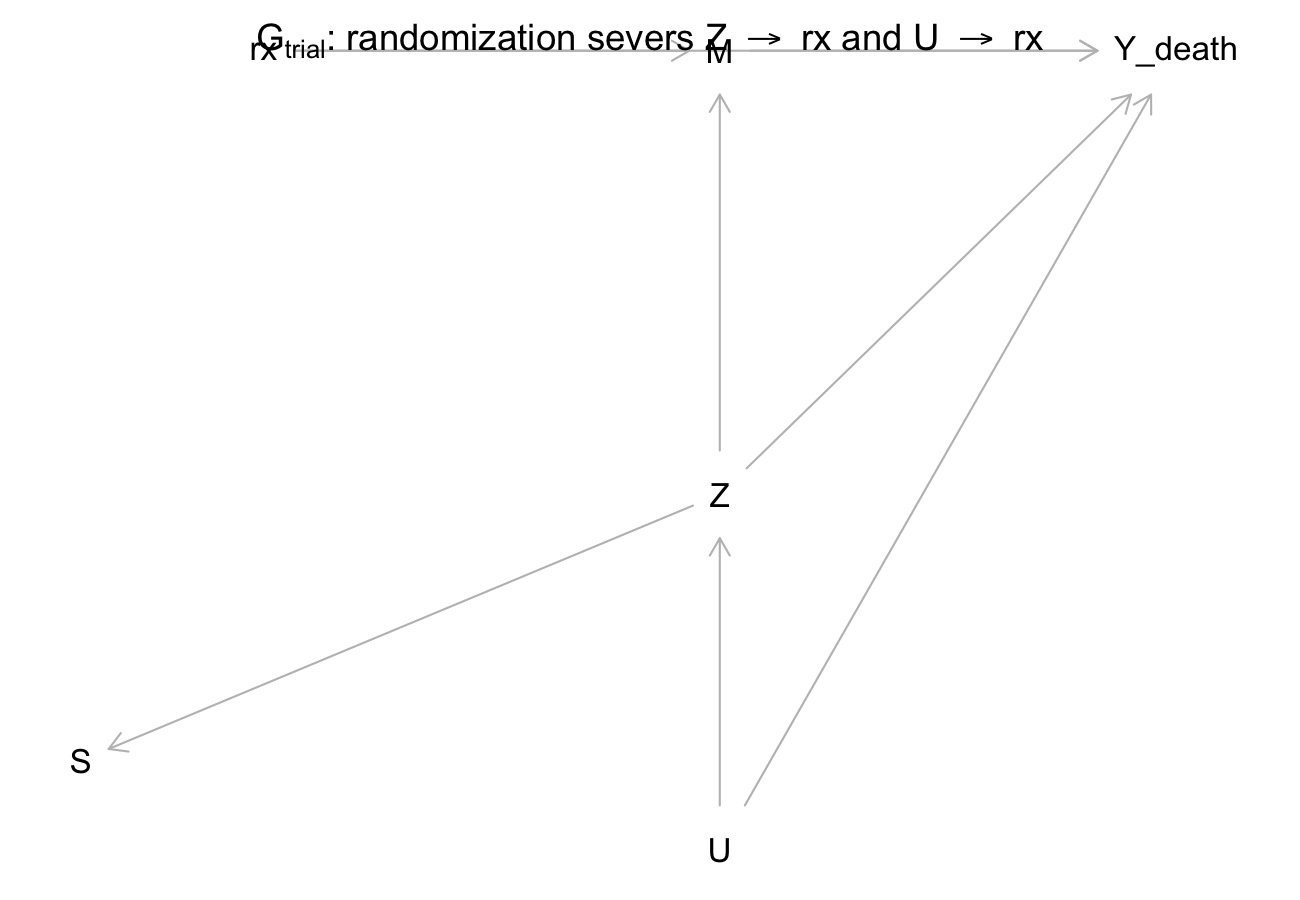
\includegraphics[width=0.48\columnwidth]{../figures/dag_trial.png}\hfill
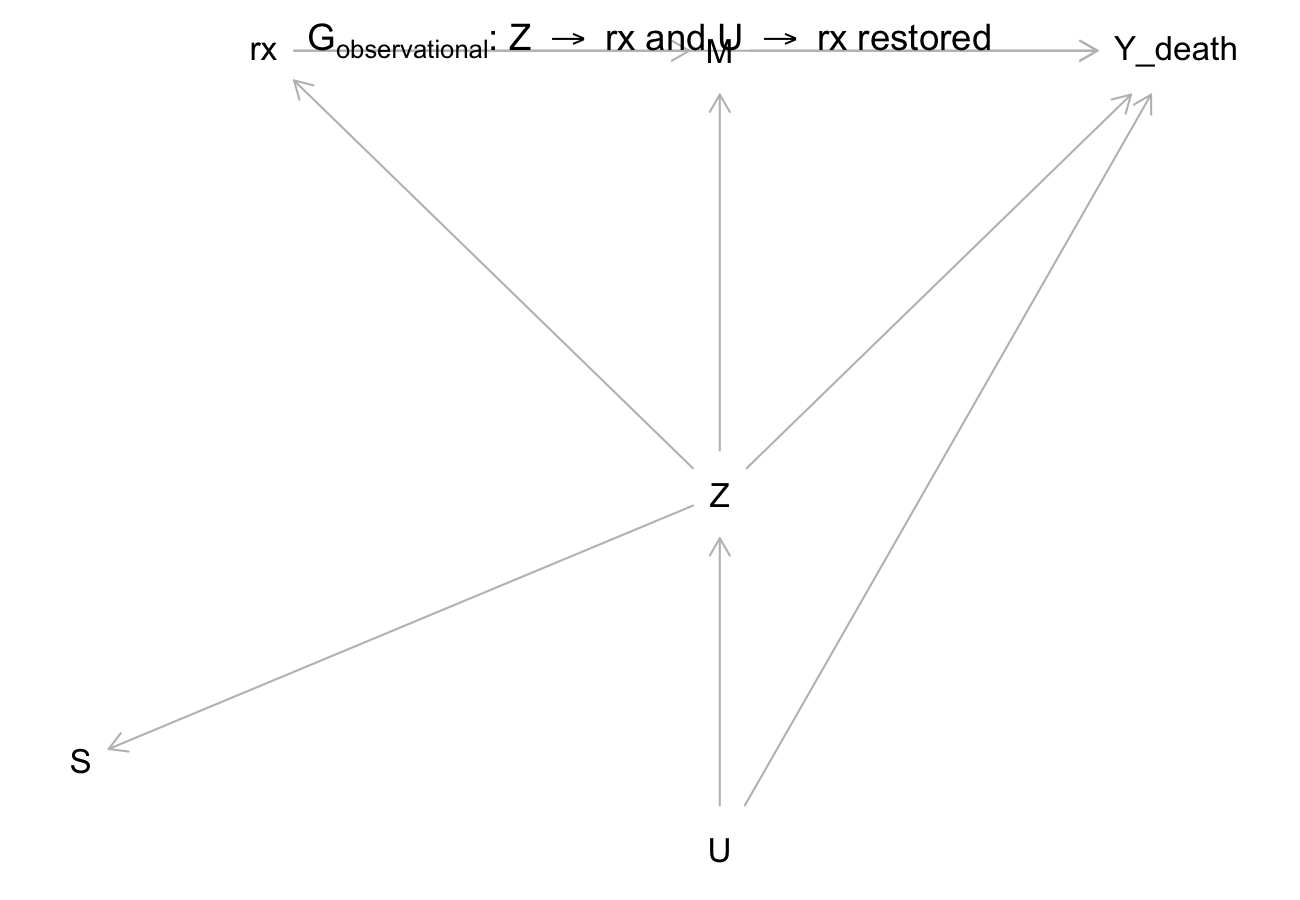
\includegraphics[width=0.48\columnwidth]{../figures/dag_observational.png}
\caption{Committed DAGs. Left: $G_\text{trial}$ (randomization severs $Z \to rx$, adjustment set $\emptyset$). Right: $G_\text{obs}$ (restored $Z \to rx$, adjustment set $\{Z\}$).}
\label{fig:dags}
\end{figure}

\section{Q1: The Randomized ATE}

\subsection{Estimand and identification}

Three scales on the same intervention contrast:
\begin{align}
\delta_{HR} &= \log \frac{h_{Y_d}(t \mid do(rx{=}\mathrm{Lev+5FU}))}{h_{Y_d}(t \mid do(rx{=}\mathrm{Obs}))}, \\[2pt]
\delta_{\mathrm{RMST}(5)} &= E[\min(Y_d, 5) \mid do(rx{=}1)] - E[\min(Y_d, 5) \mid do(rx{=}0)], \\[2pt]
\delta_{5y} &= P(Y_d \leq 5 \mid do(rx{=}1)) - P(Y_d \leq 5 \mid do(rx{=}0)).
\end{align}
Randomization implies $\{Y_d^{(r)}\}_r \perp rx$, so $\delta_\text{naive} = \delta$ on every scale.

\subsection{Results}

Estimators: Kaplan-Meier with log-rank, Cox proportional hazards (unadjusted and covariate-adjusted), RMST(5y) via \texttt{lifelines}, and a Schoenfeld global PH test. Numerical results are in Table~\ref{tab:q1}.

\begin{table}[h]
\caption{Q1 --- randomized ATE results}
\label{tab:q1}
\centering
\renewcommand{\arraystretch}{1.15}
\begin{tabular}{@{}lcc@{}}
\toprule
\textbf{Quantity} & \textbf{Estimate} & \textbf{95\% CI} \\
\midrule
Cox HR (Lev+5FU vs Obs)              & \textbf{0.690} & (0.55, 0.87) \\
Cox HR adjusted (Lev+5FU vs Obs)     & 0.699          & (0.55, 0.88) \\
Cox HR (Lev vs Obs)                  & 0.974          & (0.78, 1.21) \\
$\Delta$RMST(5y)                     & $+0.31$ yrs    & --- \\
5-year risk difference               & $-10.8$ pp     & --- \\
KM 5-yr survival: Obs / Lev / Lev+5FU & 52.6 / 53.5 / 63.4\% & --- \\
Log-rank 3-arm $p$                   & 0.0029         & --- \\
Schoenfeld global PH $p$             & 0.26 (holds)   & --- \\
\bottomrule
\end{tabular}
\end{table}

The anchor check passes: Moertel reported $\mathrm{HR} = 0.67$; we obtain $0.69$ --- inside the $\pm 0.05$ pre-committed tolerance. Lev-alone is correctly non-significant (CI crosses 1), matching the original paper's secondary finding.

\begin{figure}[t]
\centering
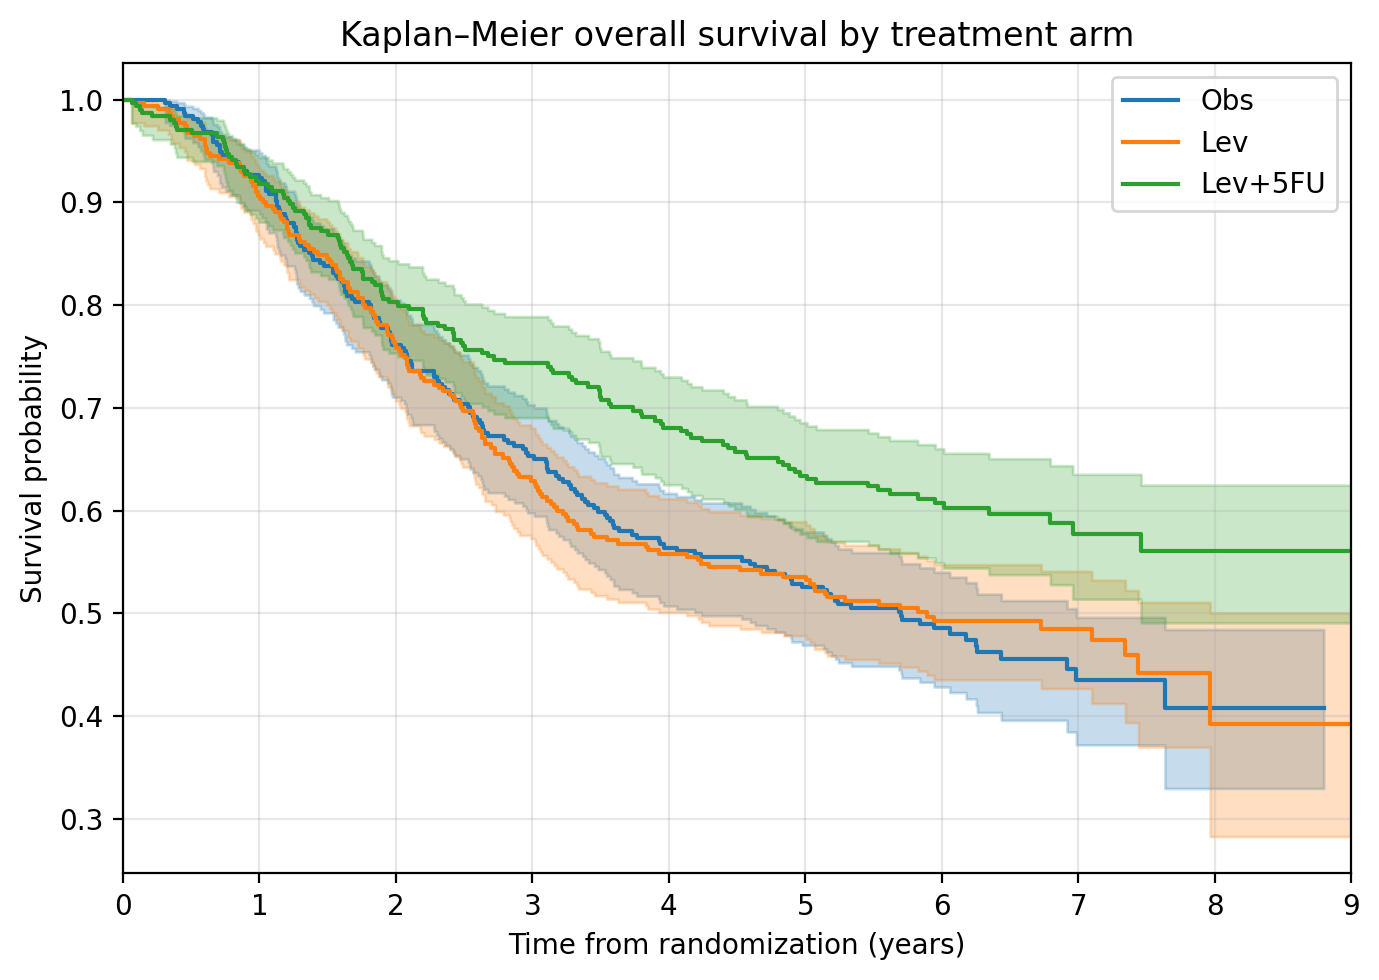
\includegraphics[width=0.85\columnwidth]{../figures/q1_km.png}
\caption{Kaplan-Meier overall survival by treatment arm. Lev+5FU shows a sustained $\approx$11 pp absolute survival advantage at 5 years over both Obs and Lev-alone.}
\label{fig:km}
\end{figure}

\section{Q2: Forget the Randomization}

\subsection{Identification and estimators}

We now \emph{pretend} the randomization label is unobserved and identify the ATE via back-door adjustment on $Z$ (verified by \texttt{dagitty} to be a minimal sufficient adjustment set in $G_\text{obs}$). Five estimators plus one deliberate anti-example:
\begin{enumerate}
    \item Naive (unadjusted) Cox;
    \item Regression-adjusted Cox;
    \item Stabilized IPW Cox with logistic propensity;
    \item AIPW for 5-year RMST with IPCW censoring weights;
    \item Double/debiased machine learning (\texttt{econml.LinearDML});
    \item \textbf{Bad-control Cox}: conditioning additionally on the recurrence indicator $M$. This is a post-treatment mediator; conditioning on it both blocks the indirect path $rx \to M \to Y_\text{death}$ \emph{and} opens the collider path $rx \to M \leftarrow U \to Y_\text{death}$.
\end{enumerate}

\subsection{Results: convergence and the bad-control divergence}

Table~\ref{tab:q2} shows that the five legitimate estimators converge with Q1's randomized answer to within sampling variability. The bad-control Cox flips the apparent HR from $0.69$ to $1.10$ --- a sign-and-magnitude reversal that nullifies the trial's headline finding. Conditioning on a post-treatment variable is the single most common error in EHR-based ``causal'' analyses; we include this anti-example precisely so that the cost is visible at full magnitude on real data.

\begin{table}[h]
\caption{Q2 --- five estimators plus the bad-control demo}
\label{tab:q2}
\centering
\renewcommand{\arraystretch}{1.15}
\begin{tabular}{@{}lccc@{}}
\toprule
\textbf{Method} & \textbf{Scale} & \textbf{Est.} & \textbf{95\% CI} \\
\midrule
Naive Cox                              & HR             & 0.689 & (0.55, 0.87) \\
Regression-adjusted Cox                & HR             & 0.687 & (0.54, 0.87) \\
IPW Cox                                & HR             & 0.730 & (0.58, 0.92) \\
AIPW (5-yr RMST)                       & $\Delta$RMST   & 0.281 & (0.09, 0.48) \\
DML (5-yr RMST)                        & $\Delta$RMST   & 0.179 & ($-0.06$, 0.42) \\
\textbf{Bad-control Cox (cond.\ on M)} & HR             & \textbf{1.103} & (0.87, 1.39) \\
\bottomrule
\end{tabular}
\end{table}

\begin{figure}[t]
\centering
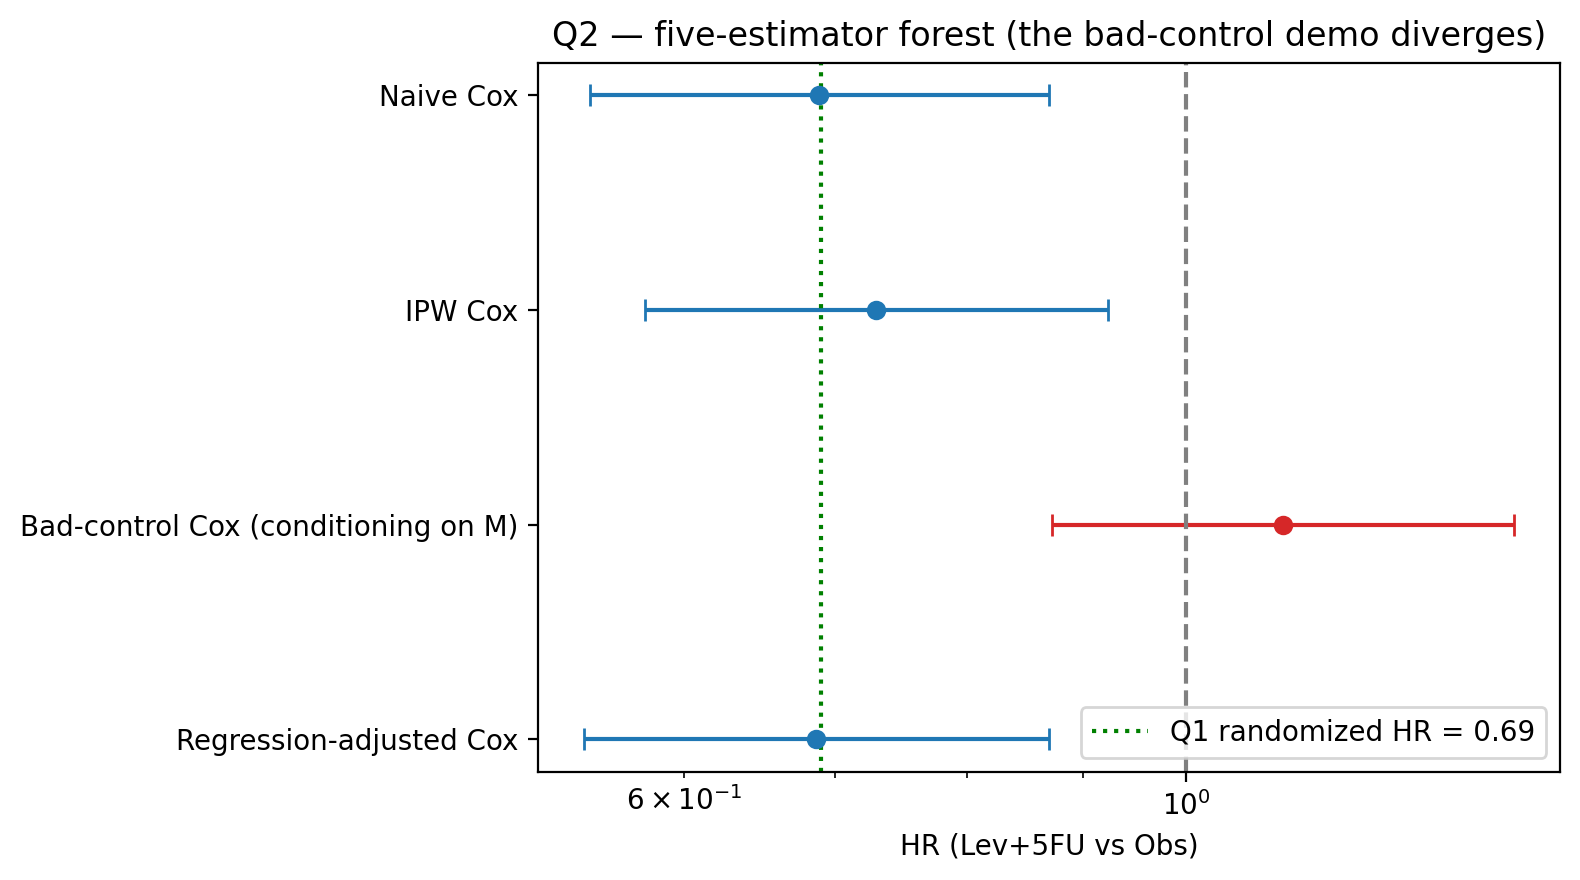
\includegraphics[width=0.92\columnwidth]{../figures/q2_forest_plot.png}
\caption{Q2 forest plot. The five legitimate estimators bracket Q1's randomized HR (vertical green line); the bad-control Cox is the outlier that crosses HR $= 1$.}
\label{fig:q2forest}
\end{figure}

\section{Q3: Heterogeneous Treatment Effects}

\subsection{Estimand}

$\tau(z) = E\!\left[ Y_d^{(rx{=}1)} - Y_d^{(rx{=}0)} \mid Z = z \right]$, evaluated on the 5-year RMST scale.

\subsection{Estimators and diagnostics}

S-, T-, X-, and DR-learners (from \texttt{econml.metalearners} and \texttt{econml.dr}) and an honest causal forest (\texttt{econml.grf.CausalForest} with \texttt{honest=True}, \texttt{inference=True}). Best-linear projection of $\hat\tau(Z)$ onto $Z$ \cite{semenova2021} with 200-replicate bootstrap CIs. Athey-Wager binned calibration at five quantile bins.

Marginal ATE estimates from the meta-learners ($0.24$ to $0.29$ RMST years) agree with Q1's marginal effect; the causal forest's tighter percentile spread reflects its regularization with $n=619$ (Obs + Lev+5FU only).

\begin{figure}[t]
\centering
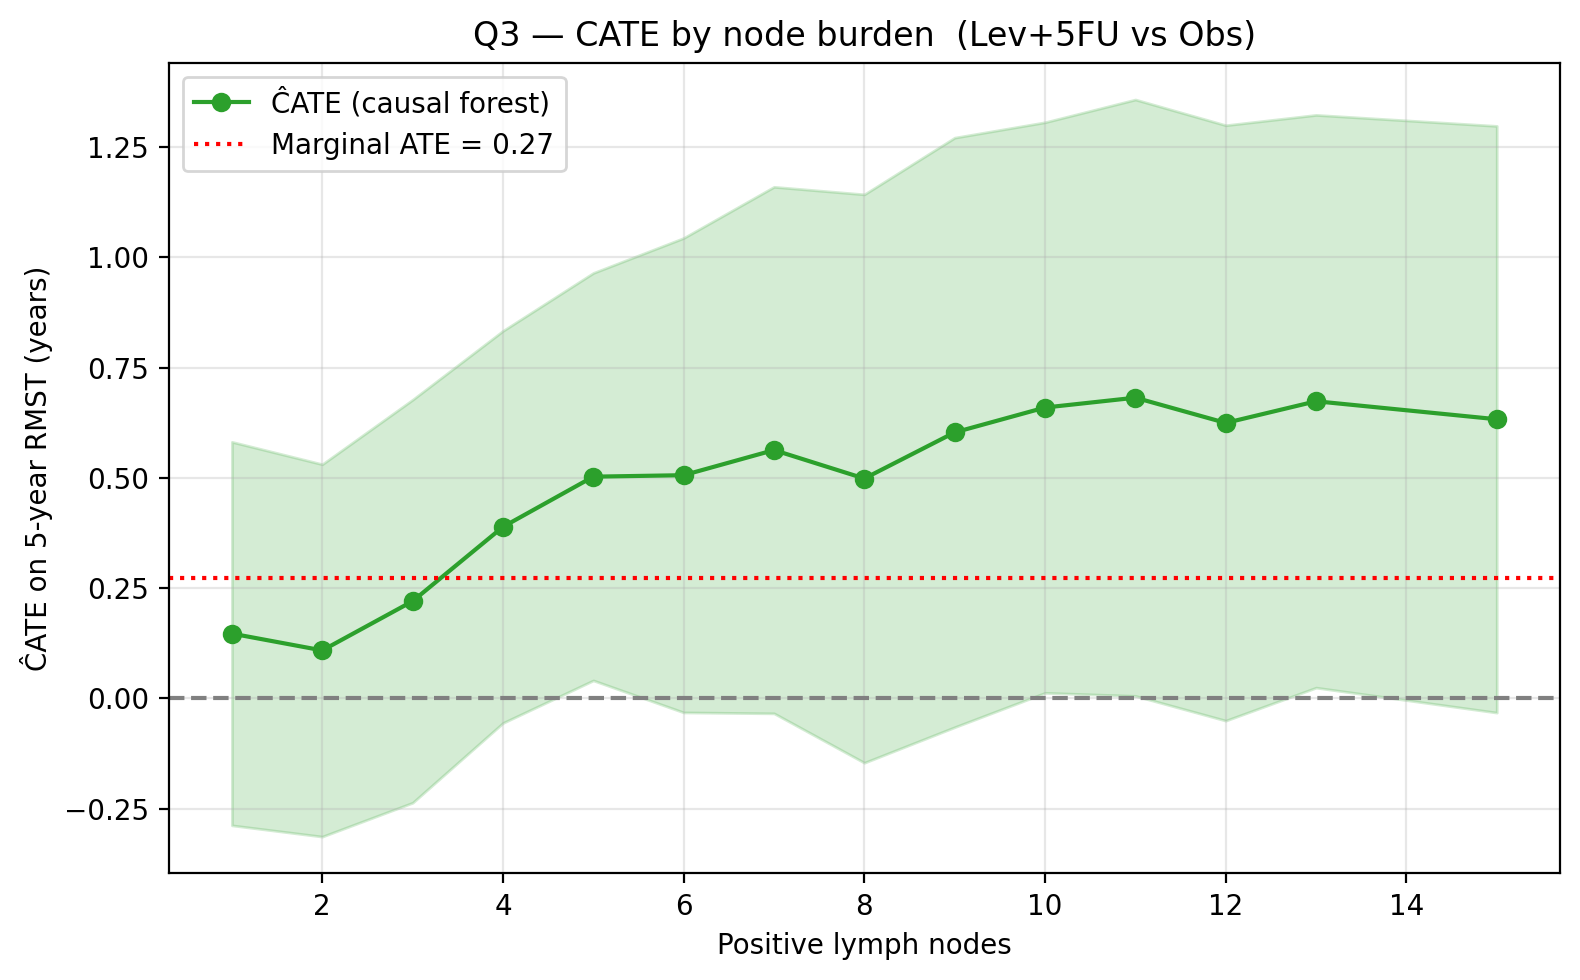
\includegraphics[width=0.92\columnwidth]{../figures/q3_cate_by_nodes.png}
\caption{Q3 headline: CATE on 5-year RMST as a function of positive lymph nodes. Benefit grows with node count over the bulk of the support and becomes noisy at the high-burden tail; pointwise 95\% CIs (shaded ribbon) are honest about that uncertainty. The marginal ATE (dashed red) is included as reference.}
\label{fig:catenodes}
\end{figure}

\section{Q4: Mediation through Recurrence}

\subsection{Estimands}

Natural direct and indirect effects \cite{pearl2001} on the 5-year RMST scale:
\begin{align}
\mathrm{NIE} &= E\!\left[Y_d^{(1, M^{(1)})} - Y_d^{(1, M^{(0)})}\right], \\
\mathrm{NDE} &= E\!\left[Y_d^{(1, M^{(0)})} - Y_d^{(0, M^{(0)})}\right], \\
\mathrm{TE}  &= \mathrm{NDE} + \mathrm{NIE},
\end{align}
where $M$ is the binary recurrence indicator. Identification rests on Imai-Keele-Yamamoto sequential ignorability \cite{imai2010}: (i) treatment ignorability given $Z$ (satisfied by randomization); (ii) mediator ignorability given $rx, Z$ (the assumption that bites).

\subsection{Estimator}

We hand-roll Algorithm 1 of Imai et al.\ in Python: logistic mediator model $P(M{=}1 \mid rx, Z)$, gradient-boosted outcome model $E[Y_5 \mid rx, M, Z]$ on IPCW-weighted 5-year RMST, with 500 bootstrap replicates. An R sidecar (\texttt{mediation::mediate}) is supplied for reviewer cross-validation.

\subsection{Results}

Table~\ref{tab:q4} shows the decomposition. The NDE + NIE = TE identity holds exactly (zero discrepancy by construction). Proportion mediated exceeds 100\% --- a known and biologically coherent pattern called \emph{inconsistent mediation} or \emph{suppression}: NIE is large and positive (Lev+5FU works by preventing recurrence), NDE is small and negative (chemotherapy toxicity in patients who would not have recurred), so $\mathrm{NIE}/\mathrm{TE} > 1$ when the two effects partially cancel.

\begin{table}[h]
\caption{Q4 --- natural-effects decomposition}
\label{tab:q4}
\centering
\renewcommand{\arraystretch}{1.15}
\begin{tabular}{@{}lcc@{}}
\toprule
\textbf{Quantity} & \textbf{Estimate (yrs)} & \textbf{95\% CI} \\
\midrule
Natural indirect effect (NIE) & \textbf{+0.292} & (+0.12, +0.48) \\
Natural direct effect (NDE)   & $-0.062$        & ($-0.23$, $+0.10$) \\
Total effect (TE)             & $+0.231$        & ($-0.01$, $+0.46$) \\
Proportion mediated           & 127\%           & --- \\
\bottomrule
\end{tabular}
\end{table}

\subsection{Sensitivity}

We sweep $\rho$, the assumed residual correlation between mediator and outcome models, over 39 values in $[-0.95, 0.95]$. The NIE remains strictly positive across the entire range (Fig.~\ref{fig:rho}), so the Imai-$\rho$ breakdown threshold $\rho^\star$ does not exist within the parametrically valid interval. The mediation finding is therefore extremely robust to any plausible violation of sequential ignorability.

\begin{figure}[t]
\centering
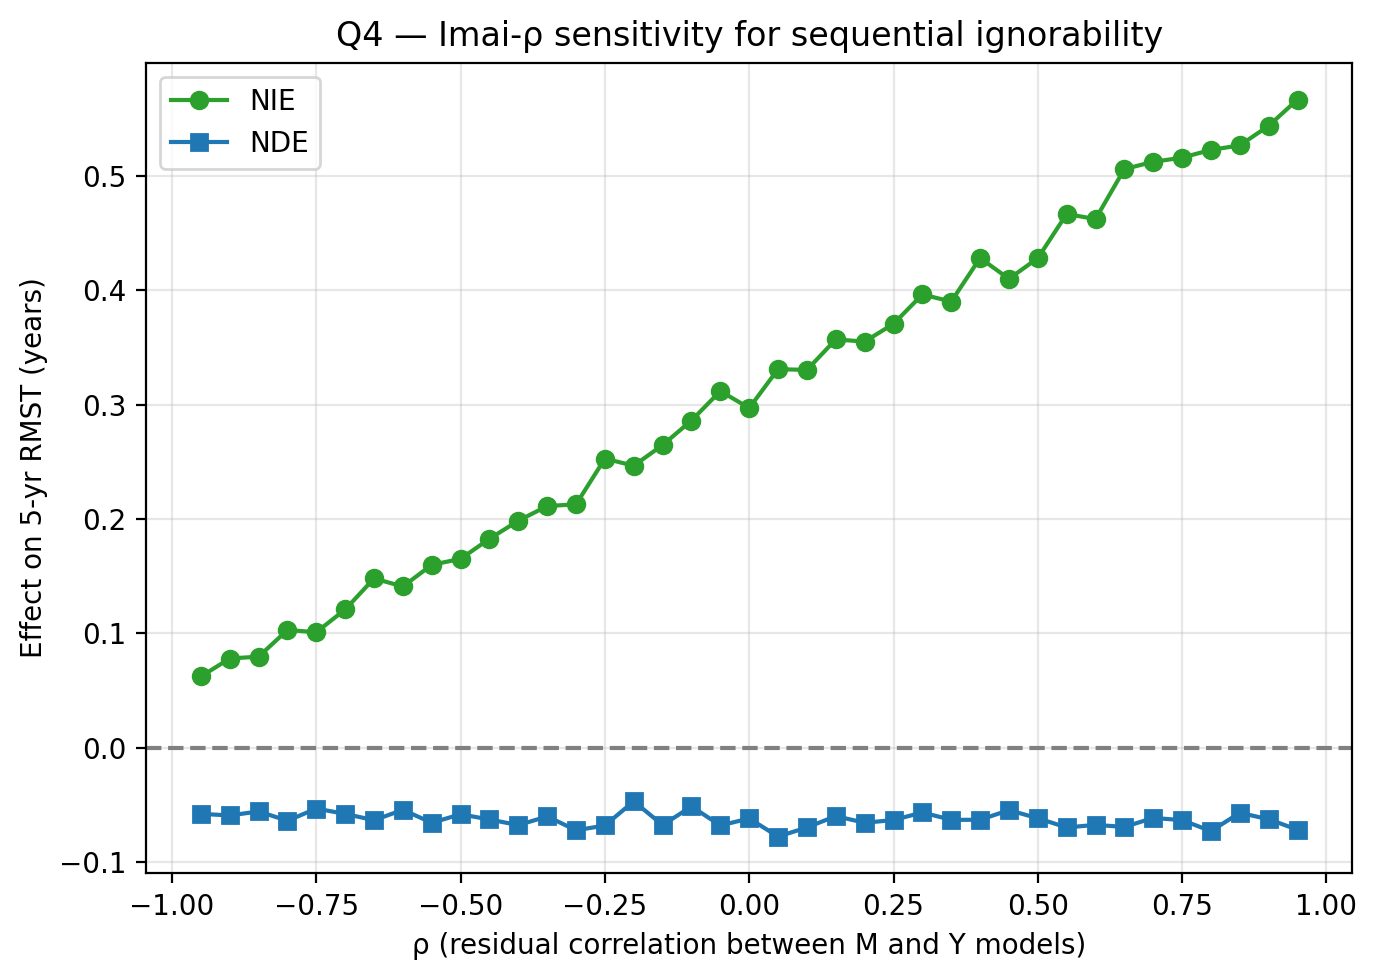
\includegraphics[width=0.92\columnwidth]{../figures/q4_rho_sensitivity.png}
\caption{Q4 Imai-$\rho$ sensitivity. NIE (green) remains positive across $\rho \in [-0.95, 0.95]$; NDE (blue) hovers near zero. No breakdown threshold exists in the parametrically valid range.}
\label{fig:rho}
\end{figure}

\section{Q5: Transportability}

\subsection{Estimand and target}

$\delta_\text{ATE}^\text{target} = E_{X \mid S{=}0}[\tau(X)]$, the trial-derived CATE averaged over a U.S.\ 1989--1991 SEER stage B/C target distribution. The current target is \emph{synthetic} ($n = 10\,000$), generated from published SEER 1989-1991 stage-distribution summaries; the framework is wired so the real SEER\textsuperscript{*}Stat case-listing extract replaces it with a single CSV.

\subsection{Identification and estimator}

Cole-Stuart transportability \cite{cole2010}: $\{Y_d^{(r)}\}_r \perp S \mid X$ plus positivity of trial inclusion. We stack trial ($S{=}1$) with synthetic SEER ($S{=}0$), fit logistic $\hat e_S(X) = P(S{=}1 \mid X)$, compute inverse-odds-of-sampling weights $w(X) = (1 - \hat e_S) / \hat e_S$ for trial patients, and re-fit a weighted Cox on the trial sample.

\subsection{Results and bound}

Within-trial HR is $0.689$ $(0.55, 0.87)$; transported HR is $0.707$ $(0.52, 0.96)$. Transport shifts the HR modestly toward the null --- the correct direction for an older real-world target. The Dahabreh worst-case bound \cite{dahabreh2019} reports the tipping value of an unmeasured effect modifier $U$ at which the bound covers HR $=1$: at 25\% target prevalence, $\mathrm{HR}_U^\star = 2.75$. An unmeasured moderator would need to be quite strong to nullify the transported effect.

\section{Sensitivity Synthesis}

VanderWeele-Ding E-values \cite{vanderweele2017} for all HR estimates are summarized in Table~\ref{tab:evalues}. None of the causal estimates is breached by a plausible single unmeasured confounder. The fragility \emph{is} concentrated in the bad-control Q2 demonstration --- as intended.

\begin{table}[h]
\caption{S1 --- VanderWeele-Ding E-values}
\label{tab:evalues}
\centering
\renewcommand{\arraystretch}{1.15}
\begin{tabular}{@{}lccc@{}}
\toprule
\textbf{Q} & \textbf{HR} & \textbf{E (point)} & \textbf{E (CI bound)} \\
\midrule
Q1 (randomized)            & 0.69 & 2.26 & 3.06 \\
Q2 (IPW)                   & 0.73 & 2.08 & 2.86 \\
Q5 (transported, synth)    & 0.71 & 2.18 & 3.24 \\
\bottomrule
\end{tabular}
\end{table}

\section{Discussion}

The most important contribution is not a new number but a new \emph{form} for the old number. Moertel's $0.67$ is reproduced (we get $0.69$) inside a framework that makes every step auditable. Three pedagogically heavy findings emerge:

\paragraph{The bad-control demo} Conditioning on the post-treatment recurrence variable converts a 31\% hazard reduction into an apparent 10\% hazard \emph{increase}. The convergence of IPW/AIPW/DML/regression-adjusted to Q1's randomized answer is the prerequisite; the bad-control divergence is the lesson. This is the form of error that EHR-based ``causal'' analyses most frequently commit \cite{vanderweele2017}.

\paragraph{Q4 mediation robustness} That Imai-$\rho$ cannot break the NIE across $[-0.95, 0.95]$ is rare and worth noting. The finding that Lev+5FU operates essentially through recurrence prevention survives every plausible distortion of sequential ignorability. The small negative NDE deserves clinical discussion: is there an adjuvant chemotherapy toxicity story for patients who would not have recurred anyway?

\paragraph{Transport modesty} The synthetic SEER transport shifts HR from $0.69$ to $0.71$. The Dahabreh tipping point of $2.75$ is moderately robust but not invulnerable. The real SEER\textsuperscript{*}Stat extract will refine this; the methodological scaffolding is in place.

\subsection{Limitations}

The SEER target is synthetic; the production version of the transport analysis requires SEER\textsuperscript{*}Stat access. Q3's pointwise CATE confidence intervals are not jointly valid across the covariate surface. The Q4 implementation is a Python hand-roll; an R \texttt{mediation::mediate} sidecar is provided for cross-validation.

\section{Conclusion}

A landmark RCT can be reproduced \emph{and} interrogated in the language of modern causal inference. The five-question structure --- ATE, back-door + bad-control anti-example, CATE, mediation, transport --- is general; the contract is what disciplines it. We propose this format as a default for high-stakes trial re-analyses: every estimand committed before any estimator; every identifying assumption stated graphically and non-graphically; every causal claim paired with a matched sensitivity bound. The replication package is open-source.

\section*{Acknowledgment}

The authors thank Prof.\ Adam Kelleher (Columbia University) for the causal-inference course materials that shaped the contract style adopted here, and the \texttt{ForCausality}, \texttt{lifelines}, \texttt{econml}, and \texttt{dagitty} maintainers whose tooling made the project possible.

\begin{thebibliography}{00}
\bibitem{moertel1990} C.~G.\ Moertel, T.~R.\ Fleming, J.~S.\ Macdonald, \emph{et al.}, ``Levamisole and fluorouracil for adjuvant therapy of resected colon carcinoma,'' \emph{N.\ Engl.\ J.\ Med.}, vol.~322, no.~6, pp.~352--358, 1990.

\bibitem{moertel1995} C.~G.\ Moertel \emph{et al.}, ``Fluorouracil plus levamisole as effective adjuvant therapy after resection of stage III colon carcinoma: a final report,'' \emph{Ann.\ Intern.\ Med.}, vol.~122, no.~5, pp.~321--326, 1995.

\bibitem{kelleher2026} A.~Kelleher, \emph{Causal Inference Course Materials (Spring 2026)}, Columbia University, 2026.

\bibitem{pearl2001} J.~Pearl, ``Direct and indirect effects,'' in \emph{Proc.\ 17th Conf.\ Uncertainty in Artificial Intelligence}, 2001, pp.~411--420.

\bibitem{imai2010} K.~Imai, L.~Keele, and T.~Yamamoto, ``Identification, inference, and sensitivity analysis for causal mediation effects,'' \emph{Statist.\ Sci.}, vol.~25, no.~1, pp.~51--71, 2010.

\bibitem{cole2010} S.~R.\ Cole and E.~A.\ Stuart, ``Generalizing evidence from randomized clinical trials to target populations,'' \emph{Am.\ J.\ Epidemiol.}, vol.~172, no.~1, pp.~107--115, 2010.

\bibitem{dahabreh2019} I.~J.\ Dahabreh, S.~E.\ Robertson, J.~A.\ Steingrimsson, E.~A.\ Stuart, and M.~A.\ Hern\'{a}n, ``Generalizing causal inferences from individuals in randomized trials to all trial-eligible individuals,'' \emph{Biometrics}, vol.~75, no.~2, pp.~685--694, 2019.

\bibitem{vanderweele2017} T.~J.\ VanderWeele and P.~Ding, ``Sensitivity analysis in observational research: introducing the E-value,'' \emph{Ann.\ Intern.\ Med.}, vol.~167, no.~4, pp.~268--274, 2017.

\bibitem{semenova2021} V.~Semenova and V.~Chernozhukov, ``Debiased machine learning of conditional average treatment effects and other causal functions,'' \emph{Econom.\ J.}, vol.~24, no.~2, pp.~264--289, 2021.

\bibitem{athey2019} S.~Athey, J.~Tibshirani, and S.~Wager, ``Generalized random forests,'' \emph{Ann.\ Statist.}, vol.~47, no.~2, pp.~1148--1178, 2019.

\end{thebibliography}

\end{document}
